\documentclass[11pt]{article}
\usepackage[margin=1in]{geometry}
\usepackage{amsmath,amssymb}
\usepackage{booktabs}
\usepackage{array}
\usepackage{graphicx}
\usepackage{xcolor}
\usepackage[colorlinks=true,linkcolor=blue,urlcolor=blue]{hyperref}
\usepackage{enumitem}
\usepackage{tcolorbox}
\usepackage[T1]{fontenc}

\newcommand{\code}[1]{\texttt{#1}}
\newcommand{\lam}{\lambda}
\newcommand{\lamf}{\lambda_f}
\newcommand{\Sig}{\Sigma^{2}}
\newcommand{\nh}{\hat{n}}
\newcommand{\D}{D}
\newcommand{\E}{\mathbb{E}}
\newcommand{\Cov}{\mathrm{Cov}}
\setlength{\parindent}{0pt}
\setlength{\parskip}{4pt}

\title{\vspace{-2.5em}MC Sachs two-point: numerical quantities, definitions,\\
and comparison with analysis-3}
\author{\code{analyses/mc\_sachs\_2pt/} \quad (internal reference)}
\date{2026-06-06}

\begin{document}
\sloppy
\maketitle
\vspace{-1.5em}

Every quantity is given with its exact mathematical definition and the code symbol
that implements it. Lengths are physical Mpc; the affine parameter $\lam$ is $0$ at
the observer and increases toward the source $\lamf$. Component convention:
$s=(s_0,s_1,s_2)=(\Phi_{00},\,\mathrm{Re}\,\Psi_0,\,\mathrm{Im}\,\Psi_0)
=(\kappa\text{-rate},\,\gamma_+\text{-rate},\,\gamma_\times\text{-rate})$. A two-ray
bundle uses $\nh_1,\nh_2$ with $\nh_1\!\cdot\!\nh_2=\cos\gamma$; the 6-vector is
$f=(f(\nh_1),f(\nh_2))$, indices $0$--$2$ = ray 1, $3$--$5$ = ray 2.

\section{Dynamics and the observable}
Stochastic Sachs fluctuation ODE (per ray; $F$ is the local quadratic vertex):
\begin{equation}
\frac{d s_a}{d\lam} = -2\,\theta_{sa}(\lam)\,s_a + F_{abc}\,s_b s_c + f_a(\nh,\lam).
\label{eq:sachs}
\end{equation}
Convergence/shear observable (the \code{integrate\_over='all'} observable):
\begin{equation}
\kappa_a(\nh) = \int_0^{\lamf} s_a(\nh,\lam)\,d\lam .
\label{eq:kappa}
\end{equation}
F-vertex (paper Table~1 $=$ \code{inputs/F\_tensor.npy}; nonzero entries)
\begin{equation}
F_{000}=-1,\;\; F_{011}=-1,\;\; F_{022}=-1,\;\; F_{101}=-2,\;\; F_{202}=-2,
\label{eq:Fvertex}
\end{equation}
so $F_{abc}s_b s_c=\bigl(-(s_0^2+s_1^2+s_2^2),\,-2s_0 s_1,\,-2s_0 s_2\bigr)$
(\code{\_F}, \code{\_f\_vertex}). The 2-point observable is the cross-ray
correlation $\xi_{ab}(\gamma)=\langle\kappa_a(\nh_1)\kappa_b(\nh_2)\rangle$; every
estimator returns this $(3,3)$ cross-ray block.

\section{Background quantities \quad{\normalsize(\code{background.py} over
\code{D\_callable.py})}}
\begin{center}
\renewcommand{\arraystretch}{1.5}
\begin{tabular}{@{}lll@{}}
\toprule
Quantity & Definition & Code \\ \midrule
Jacobi amplitude & $\D(\lam)=a(\lam)\,\chi(\lam)$ (flat FLRW closed form) & \code{Background.D} \\
Focusing rate & $\theta_{sa}(\lam)=\dfrac{d\ln \D}{d\lam}=\D'/\D$ & \code{Background.theta\_sa} \\
Linear response & $R(t,\lam')=\Theta(t-\lam')\,[\D(\lam')/\D(t)]^2$ & \code{Background.response\_R} \\
LOS window & $W(\lam)=\displaystyle\int_\lam^{\lamf}\!\Bigl[\tfrac{\D(\lam)}{\D(t)}\Bigr]^2 dt
=\int_\lam^{\lamf}\! R(t,\lam)\,dt$ & \code{driver\_stats.order0\_window} \\
\bottomrule
\end{tabular}
\end{center}
$R$ is the exact Green's function of the linear ($F{=}0$) part of \eqref{eq:sachs}:
$\partial_t R=-2\theta_{sa}(t)R$, $R(\lam',\lam')=1$. The linear solution is
$s^{(1)}_a(\nh,\lam)=\int_0^\lam R(\lam,\lam')f_a(\nh,\lam')d\lam'$, so from
\eqref{eq:kappa} $\kappa^{(1)}_a(\nh)=\int_0^{\lamf}W(\lam')f_a(\nh,\lam')d\lam'$:
$W$ is the window with which the observable sees a driving-field impulse. Cosmology
(hardcoded in \code{D\_callable}): flat $\Lambda$CDM, $\Omega_m=0.31609$, $h=0.6711$,
$z_s=5\Rightarrow\lamf=2313.029$ (analysis-3 baseline).

\section{Bare driving-field cumulants \quad{\normalsize(\code{driver\_stats.py})}}
The driving field is white in $\lam$ with angular cumulant densities.

\subsection{2-cumulant $\Sig$ \quad(\code{Sigma2Builder}, \code{sigma2\_matrix})}
\begin{equation}
\langle f_a(\nh_1,\lam)\,f_b(\nh_2,\lam')\rangle_c
=\Sig_{ab}(\nh_1\!\cdot\!\nh_2;\lam)\,\delta(\lam-\lam').
\label{eq:sig2def}
\end{equation}
$\Sig$ is obtained by \emph{de-windowing} the corr-op propagator
$C_{ab}(\cos;\lam_1,\lam_2)=\langle\Phi_a(\nh_1,\lam_1)\Phi_b(\nh_2,\lam_2)\rangle$
(the $R$-windowed 2-cumulant). Since $R=[\D/\D]^2$ is scalar,
\begin{equation}
\Sig_{ab}(\cos;\lam)=\D(\lam)^{-4}\,\frac{d}{d\lam}
\bigl[\D(\lam)^4\,C_{ab}(\cos;\lam,\lam)\bigr],
\label{eq:dewindow}
\end{equation}
the exact inverse of $C_{ab}(\cos;t,t)=\int_0^t[\D(\ell)/\D(t)]^4\Sig_{ab}(\cos;\ell)\,d\ell$.
\code{Sigma2Builder.matrix} splines $\D^4 C_{ab}(t,t)$ and differentiates; the
optional anchor $C_0=1/0.881=1.135$ (\code{apply\_c0}) rescales $\Sig$ so the
white-noise Order-0 matches analysis-3 in absolute normalization. The two-ray
$(6,6)$ matrix \code{sigma2\_6x6} uses within-ray ($\cos{=}1$) diagonal blocks and
cross-ray ($\cos{=}\cos\gamma$) off-diagonal blocks.

\subsection{Order-0 analytic prediction $O_0$ \quad(\code{order0\_mc})}
The linear ($F{=}0$) limit of $\langle\kappa\kappa\rangle$; \eqref{eq:sig2def}
collapses the double LOS integral to one:
\begin{equation}
O_0^{ab}(\gamma)=\int_{\lam_{\min}}^{\lamf}\Sig_{ab}(\cos\gamma;\lam)\,W(\lam)^2\,d\lam ,
\qquad \lam_{\min}=406 .
\label{eq:O0}
\end{equation}
This is the MC's \emph{exact} linear target.

\subsection{3-cumulant $\zeta$ \quad(\code{zeta\_tensor}, \code{zeta6})}
Equal-time third cumulant (delta-correlated in $\lam$):
\begin{equation}
\langle f_a(\nh_1,\lam)f_b(\nh_2,\lam')f_c(\nh_3,\lam'')\rangle_c
=\zeta_{abc}(\nh_1,\nh_2,\nh_3;\lam)\,\delta(\lam-\lam')\delta(\lam-\lam'').
\label{eq:zeta}
\end{equation}
\code{zeta\_tensor} wraps the project \code{equal\_time\_limber} $\kappa^{(3)}$
vertex: a symmetric $(3,3,3)$ tensor indexed by the cosine-triple
$(\nh_i\!\cdot\!\nh_j)$ and $\lam$ (non-$R$-contracted, lambda-density).

\subsection{Skewness deformation $Q$ \quad(\code{solve\_Q})}
For a node covariance $M^2$ and a target node 3-cumulant $Z$, solve
\begin{equation}
Z_{abc}=Q_{amn}M^2_{mb}M^2_{nc}+Q_{bmn}M^2_{ma}M^2_{nc}+Q_{cmn}M^2_{ma}M^2_{nb},
\label{eq:solveQ}
\end{equation}
for $Q$ symmetric in its last two indices (reduces to the scalar $Q=z/(3m^2)$).

\section{Monte-Carlo engine \quad{\normalsize(\code{sachs\_mc\_core.py})}}

\subsection{Exact-propagator discretization}
Uniform grid $\lam_k=\lam_{\min}+k\,d\lam$, $d\lam=(\lamf-\lam_{\min})/(N-1)$,
$\lam_{\min}=406$. Response applied \emph{into} node $k$, then drift $+$ noise
injected with unit response:
\begin{align}
\mathrm{resp}[k]&=[\D(\lam_{k-1})/\D(\lam_k)]^2,\quad \mathrm{resp}[0]=1,
\label{eq:resp}\\
s_k&=\mathrm{resp}[k]\,s_{k-1}+\bigl(F_{abc}s_b s_c\bigr)\big|_{k-1}\,d\lam+(\text{noise})_k,
\label{eq:update}\\
\kappa&=\sum_k w_k\,s_k,\quad w_k=d\lam\ (\tfrac12 d\lam\ \text{at }k=0,N{-}1)\ \text{[trapezoid]}.
\label{eq:trap}
\end{align}
(\code{\_step}, \code{\_precompute}, \code{\_field\_precompute}). With $F{=}0$,
\eqref{eq:update} telescopes to $s_k=\sum_{j\le k}[\D(\lam_j)/\D(\lam_k)]^2 dW_j$,
so the Gaussian MC reproduces \eqref{eq:O0} by construction.

\subsection{Noise models}
\textbf{White} (\code{\_precompute}; used by \code{simulate}, \code{simulate\_ff\_crn}):
the increment $dW_k$ is Gaussian with $\Cov(dW_k)=\Sig_{6\times6}(\cos\gamma;\lam_k)\,d\lam$.

\textbf{Colored AR(1)} (\code{\_field\_precompute}; used by the FK estimators): a
field with stationary node covariance and correlation length $\sigma_\lam$,
\begin{equation}
V_k=\frac{\Sig_{6\times6}(\cos\gamma;\lam_k)}{2\sigma_\lam},\quad
\rho=e^{-d\lam/\sigma_\lam},\quad
z_k=\rho z_{k-1}+\sqrt{1-\rho^2}\,L_k\xi_k,\ \ L_kL_k^{\!\top}=V_k,
\label{eq:ar1}
\end{equation}
injected as $(\text{noise})_k=f_k\,d\lam$. The factor $1/(2\sigma_\lam)$ enforces
$\int\langle z(\lam)z(\lam')\rangle\,d\Delta=2\sigma_\lam V=\Sig$ (one-delta
collapse), recovering the white density \eqref{eq:sig2def} as $\sigma_\lam\to0$.

\textbf{Skew injection} (\code{skew\_scale}$\neq0$): deform by a local quadratic,
\begin{equation}
f_{s,k}=z_k+\tfrac12\,Q_k\bigl(z_k\otimes z_k-V_k\bigr),\quad
Q_k=\text{skew}\cdot\code{solve\_Q}\!\Bigl(V_k,\ \tfrac{\zeta_{6,k}}{(2\sigma_\lam)^2}\Bigr).
\label{eq:skew}
\end{equation}
The node target $\mu_{3,k}=\zeta_{6,k}/(2\sigma_\lam)^2$ (two-delta collapse) gives
$\iint\langle f_s f_s f_s\rangle\,d\Delta_1 d\Delta_2=\zeta_{6,k}$, reproducing
\eqref{eq:zeta}. Note $Q_k\sim\zeta_6/(3(\Sig)^2)\sim-1.4\!\times\!10^7$ is
$\sigma_\lam$-\emph{independent}; the field skewness $\sim\zeta_{6,\rm node}/V^{3/2}
\sim4$--$6$ grows as $\sigma_\lam^{-1/2}$ (L\'evy).

\section{Channels and estimators}
The MC yields only \emph{full} (all-orders-in-$F$) correlations, each compared to
the sft-wick partial sum truncated at order~2.

\textbf{(a) Gaussian full} (\code{simulate}): white, $F$ on, no skew;
$\xi=\bigl[(1/N_{\rm good})\sum\kappa\otimes\kappa\bigr]_{[0{:}3,\,3{:}6]}$. Contains
$O_0+\mathrm{FF}+\dots$; \code{o0\_analytic}$=$\eqref{eq:O0}.

\textbf{(b) FF via $F$-toggle CRN} (\code{simulate\_ff\_crn}): two arms share the
\emph{same} white noise, $F$ on vs off, differenced per realization:
\begin{align}
\mathrm{FF}^{\rm mom}_{ab}&=\langle\kappa_a\kappa_b\rangle_{F\text{-on}}
-\langle\kappa_a\kappa_b\rangle_{F\text{-off}},
\label{eq:ffmom}\\
\mathrm{FF}^{\rm disc}_{ab}&=\langle\kappa_a\rangle_{F\text{-on}}\langle\kappa_b\rangle_{F\text{-on}}
-\langle\kappa_a\rangle_{F\text{-off}}\langle\kappa_b\rangle_{F\text{-off}},
\label{eq:ffdisc}\\
\mathrm{FF}^{\rm conn}_{ab}&=\mathrm{FF}^{\rm mom}_{ab}-\mathrm{FF}^{\rm disc}_{ab}.
\label{eq:ffconn}
\end{align}
Since $\langle\kappa\rangle_{F\text{-off}}=0$, $\mathrm{FF}^{\rm disc}=\langle\kappa\rangle_2
\otimes\langle\kappa\rangle_2$, the square of the mean 2nd-order convergence
$\langle\kappa\rangle_2=\int W\,F_{abc}\langle s_b s_c\rangle$.

\begin{figure}[htbp]
\centering
\includegraphics[width=\linewidth]{figures/ff_channel_mc_vs_analysis3.pdf}
\caption{FF channel (Task 1): the FULL FF moment, MC vs analysis-3 (no
connected/disconnected split). \emph{Left:} analysis-3 FF (line) vs the MC
$F$-on/off CRN moment (markers, anchor off), with O0 for context. \emph{Right:}
the ratio rises from $\sim0.87$ (small $\gamma$) to $\sim0.94$ (large $\gamma$) --
the equal-time (white-noise) approximation of the 2-cumulant, the same
finite-$\lambda$-correlation behind the O0 anchor $0.881$, larger at small $\gamma$
(where FF $\sim(\Sig)^2$) and smaller at large $\gamma$ (where the
$\gamma$-independent, exactly-de-windowed diagonal variance dominates).}
\label{fig:ff}
\end{figure}

\textbf{(c) Analytic equal-time FK} (\code{fk\_analytic.py}). The order-2 FK diagram
(one $F$-vertex, one $\zeta$) has four $R$-propagators and zero $C$:
obs$_a\!\xrightarrow{R}\!F\xrightarrow{R,R}$ two $\zeta$ legs;
third $\zeta$ leg $\xrightarrow{R}$ obs$_b$. The two $F$-side legs are co-located on
$\nh_a$ (triple $(1,\cos\gamma,\cos\gamma)$); the equal-time $\delta$ of
\eqref{eq:zeta} collapses the 4-D time integral to 2-D, and
\code{integrate\_over='all'} turns each external $R$ into $W$:
\begin{equation}
\boxed{\;\xi^{\rm FK}_{ab}(\gamma)=\int_0^{\lamf}\!\!d\tau\int_0^{\tau}\!\!d\lam_v\;
W(\tau)\,W(\lam_v)\,\Bigl[\tfrac{\D(\lam_v)}{\D(\tau)}\Bigr]^{4}
G_{ab}(\lam_v;\gamma)\;}
\label{eq:fkana}
\end{equation}
\begin{equation}
G_{ab}=(M+M^{\!\top})_{ab},\qquad M_{ab}=\sum_{m,n}F_{amn}\,Z_{bmn},\qquad
Z=\zeta\bigl(\nh_1,\nh_1,\nh_2;\lam_v\bigr).
\label{eq:Gtensor}
\end{equation}
The external index $a$ rides the $F$-vertex ($F_{amn}$), only $b$ rides one $\zeta$
leg ($Z_{bmn}$); $M+M^{\!\top}$ is the $\nh_1\!\leftrightarrow\!\nh_2$ symmetrization;
the MSR/combinatorial prefactor is $1$ (calibrated on the validated demo2 integrator).
For $\kappa\kappa$: $G_{00}=-2(\zeta_{\rm TTT}+\zeta_{\rm Bmod})$. Code reduces
\eqref{eq:fkana} to two 1-D quadratures via $u=\D/\D(\lamf)$:
$\xi^{\rm FK}_{ab}=\int d\lam_v\,W u^4 G_{ab}\,H$, $H(\lam_v)=\int_{\lam_v}^{\lamf}
W(\tau)u(\tau)^{-4}d\tau$.

\begin{figure}[htbp]
\centering
\includegraphics[width=\linewidth]{figures/fk_matrix_validation.pdf}
\caption{Analytic FK \eqref{eq:fkana} vs analysis-3 over the FULL $(3,3)$ component
matrix. \emph{Left:} $|\xi^{\rm FK}_{ab}|$ vs $\gamma$ -- analytic lines, analysis-3
markers; $\gamma_+\gamma_+=\gamma_\times\gamma_\times$ (spin-2 isotropy). \emph{Right:}
the ratio is flat at $0.992$ for every nonzero pair (the $0.8\%$ is sft-wick's coarser
internal discretization), and the parity selection rule
$\xi^{\rm FK}(\kappa\gamma_\times)=\xi^{\rm FK}(\gamma_+\gamma_\times)=0$ holds exactly
in both.}
\label{fig:fkmatrix}
\end{figure}

\textbf{(d) FK Monte-Carlo, variance-reduced} (\code{simulate\_fk\_vr}). FK is linear
in $Q$, and obs$_b$ connects to its $\zeta$ leg $F$-free, so the no-$F$ windowed
response $\kappa^{(0)}_{d,B}=\int W\,\delta f_B$ suffices (no $s_d$ ODE). Pull $Q$
\emph{outside} the average:
\begin{align}
T_{AB}&=\tfrac12\,d\lam\sum_k W(\lam_k)\sum_{ij}Q_k[B,i,j]\;
C_{A,ij}(k),\quad
C_{A,ij}(k)=\Cov\!\bigl(\kappa^{F}_{g,A},\,z_i(\lam_k)z_j(\lam_k)\bigr),
\label{eq:fkmcT}\\
\mathrm{FK}_{ab}&=(T+T^{\!\top})_{[a,\,3+b]}\quad\text{(cross-ray block)}.
\label{eq:fkmc}
\end{align}
Three ingredients (all required): (i) $Q_k$ multiplies the \emph{averaged} $C$,
never the per-sample $w_{ij}=z_iz_j-V$; (ii) $C$ is the \emph{matched sample}
covariance $\langle\kappa_g z_iz_j\rangle_{\rm batch}-\langle\kappa_g\rangle\langle
z_iz_j\rangle_{\rm batch}$ (the disconnected piece is $\sim10^7\times$ the signal, so
it must be removed with the same-sample $\langle z_iz_j\rangle$, \emph{not} the
theoretical $V_k$); (iii) $\kappa^{F}_g=\kappa_g(F\text{-on})-\kappa_g(F\text{-off})$
(shared-noise CRN) drops the linear $L_1$ noise $\sim1000\times$ and fixes the sign.
The naive equivalent \code{simulate\_fk\_pathA} is blow-up-free but
statistics-hungry; kept for reference only.

\begin{figure}[htbp]
\centering
\includegraphics[width=0.62\linewidth]{figures/fk_mc_vs_analytic.pdf}
\caption{FK Monte-Carlo \eqref{eq:fkmcT} (variance-reduced, $\sigma_\lam{=}18$,
$n_\lam{=}1000$) vs the analytic equal-time FK over $\gamma$. The stochastic-Sachs
MC reproduces the analytic FK to $\sim10$--$25\%$ (ratio $\sim1.04$--$1.23$, flat),
with correct sign -- an independent confirmation of the 3-cumulant channel.}
\label{fig:fkmc}
\end{figure}

\section{Comparison with analysis-3}
Analysis-3 npz under \code{sftwick\_outputs/2PCF/}: dirs \code{C\_corr\_op\_O0},
\code{C\_corr\_op\_K\_limber\_FF}, \code{C\_corr\_op\_K\_limber\_FK}. The
$\kappa\kappa$ channel $=$ rows \code{a==0 \& b==0};
$\gamma=\deg(\arccos\hat x\!\cdot\!\hat y)\!\cdot\!60$; $\lamf=2313.029$. All inputs
($\Sig,\zeta,F,R$, observable) are the \emph{same} objects the MC uses.

\begin{figure}[htbp]
\centering
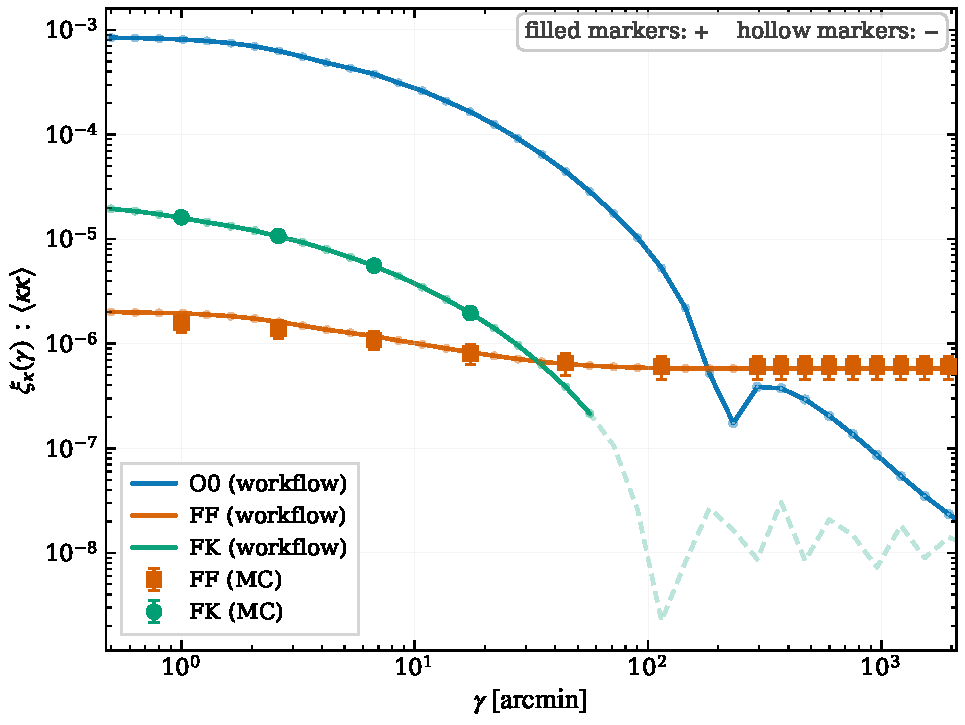
\includegraphics[width=\linewidth]{figures/xi_kappa_channels.pdf}
\caption{The convergence two-point function $\xi^{\kappa\kappa}(\gamma)$ by channel:
O0 / FF (full moment) / FK -- analysis-3 (lines) vs Monte-Carlo (markers). \emph{Left:}
O0 dominates and crosses zero ($\sim200'$); FK $\sim5\times10^{-5}$ is nearly flat;
the full FF decays toward its $\gamma$-independent large-$\gamma$ value. \emph{Right:}
channel-by-channel MC$/$analysis-3. FK $\sim1.1$ (var-reduced estimator); FF (full)
$\sim0.9$ (the equal-time deficit, rising toward $1$ at large $\gamma$); O0 is
reproduced via the anchor $0.881$. (Replaces the archived apples/oranges $F$-off
overlay.)}
\label{fig:channels}
\end{figure}

The analysis-3 tags below abbreviate the three npz directories named above.
\begin{center}
\small
\renewcommand{\arraystretch}{1.3}
\begin{tabular}{@{}>{\raggedright}p{1.1cm} >{\raggedright}p{3.0cm} >{\raggedright}p{1.4cm} p{8.0cm}@{}}
\toprule
Channel & MC quantity & analysis-3 & Result \\ \midrule
Order 0 & \code{order0\_mc}, \eqref{eq:O0} & \code{O0} &
ratio $=0.881$ ($\gamma$-indep; $C_0=1.135$ absorbs it; the $12\%$ is the
equal-time collapse dropping the cross-shell tail). \\
FF (ord.\ 2) & \code{simulate\_\allowbreak ff\_crn}, \eqref{eq:ffmom}--\eqref{eq:ffconn} &
\code{FF} (limber) &
FULL FF moment: MC$/$analysis-3 $\sim0.87$ (small $\gamma$) $\to0.94$ (large
$\gamma$), the equal-time deficit (rises as the $\gamma$-independent diagonal piece
takes over). WHY the floor: analysis-3's flat large-$\gamma$ value
$5.785\!\times\!10^{-7}$ is the disconnected $\langle\kappa\rangle_2^2$ --
code-confirmed (sft-wick FF $=5$ conn $+1$ \emph{disconnected}
$R(x,y_0)R(y,y_1)C(y_0,y_0)C(y_1,y_1)$; $\langle\kappa\rangle_2^2$ from corr-op $C$
$=$ floor to $0.5\%$). The de-windowed diagonal variance is reproduced exactly, only
the cross-shell ($\sim(\Sig)^2$) is deficient $\Rightarrow$ the $\gamma$-rising ratio. \\
FK (ord.\ 2) & \code{fk\_analytic}, \eqref{eq:fkana} & \code{FK} (limber) &
ratio $=0.992$, \emph{flat} across the full $(3,3)$ matrix (kk peak $5.449$ vs
$5.489\!\times\!10^{-5}$; parity-zero pairs $(0,2),(1,2)$ exactly $0$;
$\mathrm{FK}_{11}=\mathrm{FK}_{22}$). The $0.8\%$ is sft-wick's coarser internal
discretization (stable under refinement). \\
FK (ord.\ 2) & \code{simulate\_\allowbreak fk\_vr}, \eqref{eq:fkmcT} & via analytic &
MC$/$analytic $\sim1.04$--$1.23$ (flat over $\gamma=1'$--$114'$, SE $\sim$few \%),
sign correct. Independent stochastic-ODE confirmation to $\sim10$--$25\%$. Grid
convergence is non-monotonic (fine-grid heavy-tailed upward bias); a clean
$<10\%$ $\sigma_\lam\!\to\!0$ limit is future work. \\
\bottomrule
\end{tabular}
\end{center}

\paragraph{Consistency (doc vs code, numerically verified 2026-06-06).}
\begin{enumerate}[leftmargin=1.4em,itemsep=1pt]
\item $R(t,\lam')=[\D(\lam')/\D(t)]^2$ \quad(exact).
\item \eqref{eq:O0} lower-limit window: $W$ vs \code{scipy.quad}, rel $2\!\times\!10^{-10}$.
\item \code{order0\_mc} $=\int\Sig_{00}W^2 d\lam$ (independent quad), rel $2\!\times\!10^{-4}$.
\item \code{fk\_analytic} $=$ brute-force 2-D quadrature of \eqref{eq:fkana}, rel $2\!\times\!10^{-2}$
(coarse reference grid; confirms the integrand structure).
\item colored field $2\sigma_\lam V_{00}=\Sig_{00}$, i.e.\ $\int\langle zz\rangle d\Delta=\Sig$ \quad(exact).
\end{enumerate}
Figures (in \code{figures/}): \code{xi\_kappa\_channels} (full O0/FF/FK
decomposition, MC vs analysis-3), \code{fk\_matrix\_validation} (FK $(3,3)$ matrix
$+$ selection rules), \code{fk\_mc\_vs\_analytic} (FK MC $\gamma$-sweep),
\code{ff\_channel\_mc\_vs\_analysis3} (FF decomposition), \code{anchor\_FK\_check},
\code{anchor\_O0\_check} (all \code{.pdf}). [The earlier apples/oranges
\code{mc\_vs\_analysis3\_xi\_kappa} is archived under \code{figures/\_archive\_*}.]
Companion notes: \code{FF\_NOTES.md} (Task 1), \code{FK\_NOTES.md} (FK),
\code{DESIGN.md} (architecture).

\end{document}
